\section{TopoGen Dataset}
\label{sec:topogen}

\begin{figure*}[!t]
  \centering
  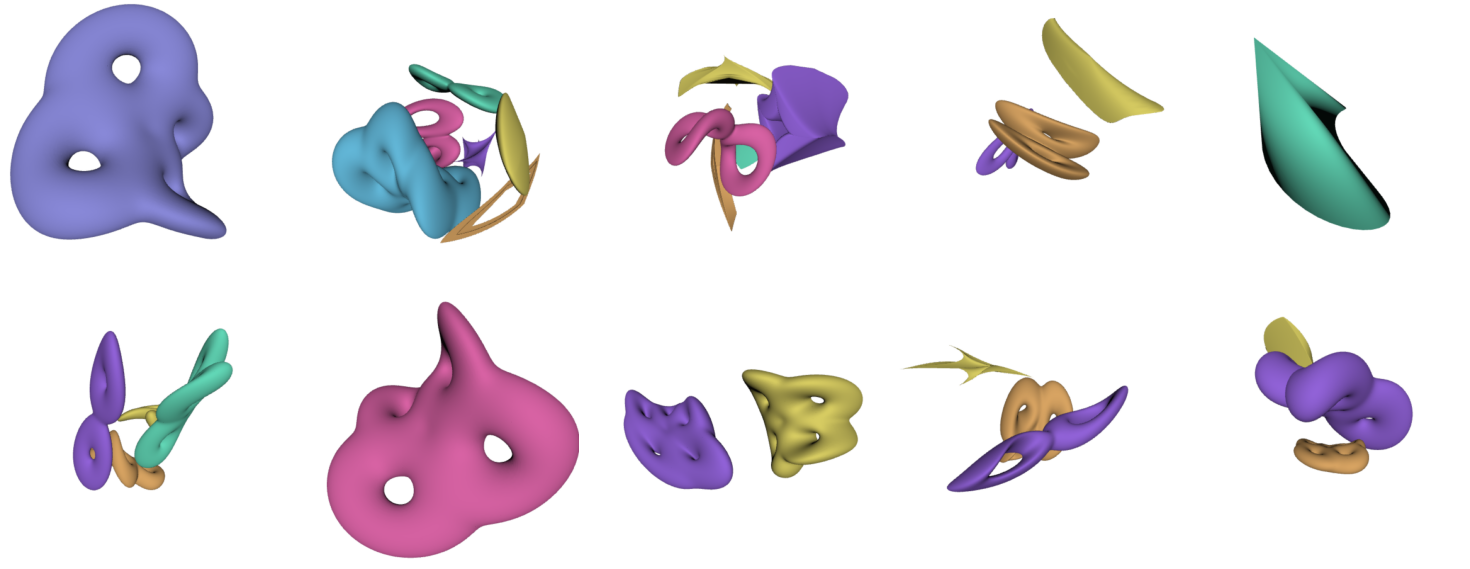
\includegraphics[width=1.0\linewidth]{figs/topogen/samples_overview.png}

  \label{fig:topogen-samples}
  \caption{\textbf{TopoGen samples.} Despite the fact that each sample is generated from a rather small family of shapes, both the topology preserving placement and augmentations allow for a rich variety of shapes, while ensuring topological consistency.}
  \label{fig:short}
\end{figure*}

Assessing how models understand the topology of 3D shapes, in particular through probing, requires data labeled with topological information and control over the distribution of the labels. However such dataset, specifically designed with a focus on the structure and not the semantics, hasn't been developed yet. Hence we introduce TopoGen, a scalable dataset of 3D synthetic shapes with accurate and well balanced topological labels. The samples in this dataset are labeled by number of connected components and genus.

\subsection{Existing datasets}
\label{ssec:existing_datasets}

When speaking about structural understanding, representations such as the ones present in the MANTRA \cite{mantra} dataset are a natural choice. The MANTRA dataset (Manifold Triangulation Assemblage) by Ballester et al. consists purely of combinatorial triangulation of 2- and 3-dimensional manifolds: i.e., its samples only include connectivity information (abstract simplicial complexes), without any geometric embedding in $\mathbb{R}^3$, making it agnostic to geometric realization. This makes MANTRA a particularly meaningful benchmark when assessing whether graph-based and simplicial complex-based models capture higher-order structures (essentially Betti numbers $\beta_0, \beta_1, \beta_2$ and $\beta_3$). However, in this work we focus on evaluating models that rely on geometric 3D representations such as meshes, point clouds, or implicit fields (e.g., Signed Distance Functions (SDFs)) (i.e., data embedded in $\mathbb{R}^3$. Therefore, MANTRA falls outside the scope of the tasks considered in this report.


Only a few large datasets have some considerations about structural information carried by meshes (commonly the number of connected components and the genus). Notably, the Thingi10K and ABC datasets, which are composed with various CAD models and artistic meshes come with such annotations. However, they turn out to be inaccurate for three reasons. 
\begin{enumerate}
  \item \textbf{Discrepancy between actual and effective number of components.} In artistic 3D modeling, a complex shape is often constructed from many mesh objects that represent fine details (buttons, ornaments, small extrusions, etc.). As a result, the true number of connected components in the mesh (counting every individual object used in the construction) can be much larger than the effective number of connected components, which corresponds to the main perceived object as a whole. (*+fig*). The same issue holds with complex CAD models.
  \item \textbf{Imbalanced annotations.} While both Thingi10K and ABC exhibit a wide range of genus values (Figure \ref{fig:thingi-genus} ADD FOR ABC), the distribution is highly imbalanced. For evaluation tasks such as probing, balanced annotations are crucial, yet in this dataset the vast majority of samples have very low genus (typically between 0 and 2), whereas high-genus shapes are severely underrepresented.
  \item \textbf{Structural artifacts.} Most meshes in these datasets are not suitable out-of-the-box for topological labelling. Many of them are non-manifold or contain self-intersecting faces. This raises two main issues. First, it makes topological analysis unreliable: for example, the Euler Characteristic (Equation \ref{eq:euler}) cannot be applied to non-manifold meshes.
\end{enumerate}
\begin{equation}
  \chi = V - E + F = 2 - 2g - b + c
  \label{eq:euler}
\end{equation}
Where $V, E, F$ are the number of vertices, edges and faces respectively, $g$ is the genus, $b$ the number of boundary components and $c$ the number of connected components.

\begin{figure}[t]
  \centering
  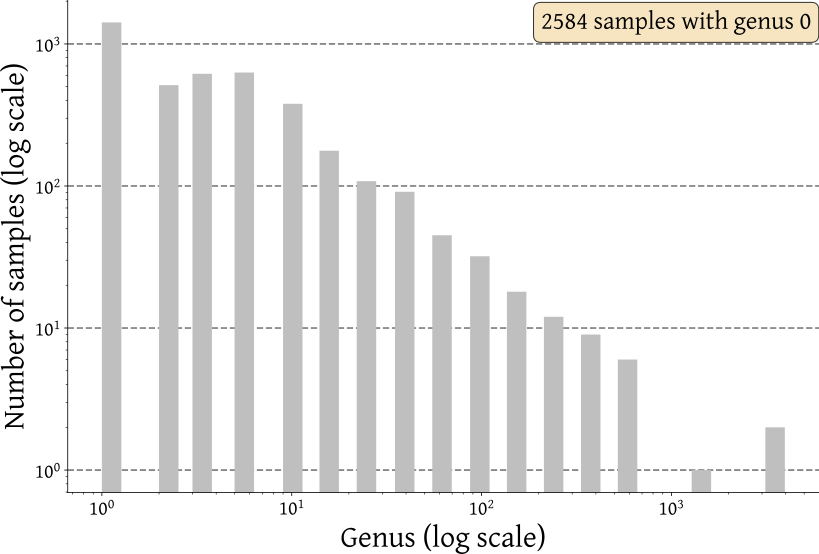
\includegraphics[width=\linewidth]{figs/topogen/thingi_genus_hist.pdf}
   \caption{\textbf{Genus distribution of Thingi10K.} Both axes are plotted in log scale. The genus was estimated from the Euler characteristic, provided as metadata with the dataset; however, 2,651 samples do not fulfill the requirements to directly compute the genus from the Euler characteristic (see \ref{eq:euler}). They are therefore not taken into account here. The histogram shows that a large fraction of the dataset (over 3,000 samples out of 7,344) has genera of 0 or 1, indicating that higher-genus components are significantly underrepresented, which may limit accurate classification and probing analyses for those cases.}
   \label{fig:thingi-genus}
\end{figure}


Second, self-intersections may introduce undesired topological structures, leading to inaccurate labels. To overcome these issues, remeshing procedures such as Manifold \cite{manifold} and ManifoldPlus \cite{manifoldplus} were proposed, transforming arbitrary meshes into manifold and watertight representations. While Manifold provides robustness, it often over smooths the input geometry, reducing fine details. ManifoldPlus improves accuracy but introduces artifacts (see Fig...) (*+example with flower pot*) in challenging cases, leading to inconsistencies in the resulting topology. More recent approaches rely on intermediate representations such as signed or unsigned distance fields. Methods like Dual Octree Graph Networks (DOGN) \cite{dogn}, and the remeshing procedure in CLAY \cite{clay} achieve more stable and reliable results, but at the cost of significantly higher computational complexity. Finally, some shapes in Thingi10K and ABC also exhibit highly uneven geometric complexity, which can negatively impact model evaluation. To ensure that results primarily reflect the topology of the shapes, a certain level of uniformity in geometric complexity across the dataset is necessary. However, quantifying geometric difficulty is challenging, as no straightforward metric exists to assess it. Moreover, since the shapes were not generated under a controlled process, it is not possible to design a general heuristic to filter out geometrically challenging samples consistently.


Finally, the EuLearn dataset (Figure \ref{fig:eulearn-samples}), intended to supervise models on inferring the genus from point clouds, offers interesting perspectives to train on synthetic data. The dataset is generated from Fourier curves with additional procedures to create knots, which in turn produce surfaces of different genera and some topological diversity. Despite its scalability in terms of the number of samples, EuLearn only covers genera between 0 and 10. Moreover, the generation rules lead to very limited variation within each genus: samples of the same class tend to look too similar, which results in strong overfitting. Figure \ref{fig:eulearn-umap-comparison} and \ref{tab:eulearn-overfit} highlight this issue at the transformer features level while Figures \ref{fig:eulearn-samples} and \ref{fig:eulearn-acc-angle} confirm this issue at the sample level. In particular, \ref{fig:eulearn-acc-angle} exhibits a strong correlation between shapes genera and their canonical orientation. Indeed, a simple nearest neighbors classifier with Chamfer distance achieves perfect accuracy on the test set if it's fit on the training set as is. Beyond this rotation-genus correlation. This correlation makes it difficult to disentangle whether classification performance is driven by topological information or by correlated geometric cues. Overall, these limitations make EuLearn unsuitable for robustly probing structural understanding in 3D shape encoders.

\begin{figure}[t]
  \centering
  \includegraphics[width=\linewidth]{figs/eulearn/dataset_samples.pdf}
   \caption{\textbf{Samples from the EuLearn dataset across different genera.} As the genus increases, shapes become geometrically more complex. This trend highlights a confounding factor in the dataset: geometric complexity grows together with genus. As a result, classification performance may be driven not only by topological information but also by correlated geometric cues.}
   \label{fig:eulearn-samples}
\end{figure}


\begin{figure}[t]
  \centering
  \includegraphics[width=\linewidth]{figs/eulearn/accuracy_vs_angle.pdf}
   \caption{\textbf{Classification accuracy vs. rotation range for KNN.} Training sets contain point clouds rotated within specified angular ranges around the z-axis. Perfect accuracy at 0rad rotation indicates exploitation of orientation-dependent features rather than robust geometric understanding. Furthermore, the dramatic drop correlated with increasing rotation range suggest a strong bias in the dataset. Ideally, we would expect the accuracy to be rather stable across different rotations. \textit{Note:} Results are cross-validated with 5 folds.}
   \label{fig:eulearn-acc-angle}
\end{figure}


\begin{figure}[t]
  \centering
  \includegraphics[width=\linewidth]{figs/eulearn/umap_comparison_original_rotated.pdf}
   \caption{\textbf{UMAP of CLS-token embeddings from Point-BERT (EuLearn dataset).} Points are colored by genus. *Left:* embeddings computed from the original provided shapes (original orientations). Samples of the same genus form tight, well-separated clusters. *Right:* the same samples, but each randomly rotated before being input to Point-BERT. Genus labels are mixed and the clusters largely disappear. However, the genus is a topological invariant. It should not be altered by any rigid transformation. If the encoder actually captured topology, we could expect the clusters to remain visible, even after rotation. Therefore, the observed genus clustering is driven by a correlation between genus and global pose / geometric complexity in EuLearn, not by robust topological features. Hence using these embeddings to probe genus is unreliable (classifiers trained on them risk exploiting pose correlation rather than true genus). Even though this doesn't strictly assess that Point-BERT doesn't capture topology, it shows at least that much of the information carried by the embeddings is not related to topology. Table ... further highlights the overfitting issue when training a linear probe on EuLearn.}
   \label{fig:eulearn-umap-comparison}
\end{figure}


\begin{figure}[t]
\centering
\begin{tabular}{c c c c}
\toprule
\textbf{Training set} & \textbf{Test set} & \textbf{Training Acc.} & \textbf{Test Acc.} \\
\bottomrule
\multirow{2}{*}{\includegraphics[height=1em]{figs/utils/unrotated.pdf}} 
  & \includegraphics[height=1em]{figs/utils/unrotated.pdf} 
  & \multirow{2}{*}{99.9} 
  & $96.4_{\textcolor{red}{(-0.5)}}$ \\
& \includegraphics[height=1em]{figs/utils/rotated.pdf} 
  &  
  & $16.3_{\textcolor{red}{(-83.6)}}$ \\
\midrule
\multirow{2}{*}{\includegraphics[height=1em]{figs/utils/rotated.pdf}} 
  & \includegraphics[height=1em]{figs/utils/rotated.pdf} 
  & \multirow{2}{*}{77.8} 
  & $50.1_{\textcolor{red}{(-27.7)}}$ \\
& \includegraphics[height=1em]{figs/utils/unrotated.pdf} 
  &  
  & $45.9_{\textcolor{red}{(-31.9)}}$ \\
\bottomrule
\end{tabular}
\caption{\textbf{Probing results on features from canonical vs. randomly rotated EuLearn samples.} 
We train linear probes on two feature sets (CLS embeddings of the last block of the Point-BERT transformer): 
(i) shapes in canonical orientation (\includegraphics[height=1em,valign=c]{figs/utils/unrotated.pdf}), and 
(ii) shapes with random 3D rotations (\includegraphics[height=1em,valign=c]{figs/utils/rotated.pdf}). 
Each probe is evaluated on test features from both canonical and rotated shapes. 
Probes trained on canonical features reach near-perfect accuracy on canonical test data but collapse under rotations, revealing overfitting to orientation. 
Probes trained on rotated features avoid this overfitting but show consistently poor generalization, with accuracy dropping by over 20\% on both canonical and rotated test sets. 
This indicates that the dataset is not suitable for robust probing of structural information.}
\label{tab:eulearn-overfit}
\end{figure}

\subsection{Method}


Since TopoGen is made of synthetic shapes, two critical challenges must be addressed to ensure that the results obtained from this dataset are relevant. 1) Foundation models are pretrained on real shapes. Therefore, learned features reflect the distribution of real world geometry and semantics. Synthetic data, however, introduce patterns and biases that don't exist in real data, making them fall out-of-distribution. 2) Another common pitfall of synthetic datasets (cf. EuLearn) is the lack of variability, making evluation tasks such as probing, trivial. In practice, the first challenge is overcome by the fact that foundation models are pre-trained on datasets (e.g ShapeNet, Objaverse, etc.) that are large enough for synthetic shapes not to fall out-of-distribution. This is experimentaly validated in Figure (+ figure with umaps). To adress the second challenge, we developed a set of rules and augmentation techniques to ensure that the generated shapes are both diverse and topologically accurate.

Below we derive these rules used to generate TopoGen, and more importantly, how the latter allow to maintain this variability across samples while scaling their number up to $10^5$ shapes.

\subsubsection{Labels Distribution}
\label{sssec:labels-distribution}

A central design choice in TopoGen is to ensure balanced topological supervision across the dataset. To this end, both the genus and the number of connected components are sampled such that their marginal distributions are approximately uniform. This prevents any single topological class from dominating and guarantees that models trained on the dataset are exposed to the full spectrum of topological structures. We bring this guarantee over marginal distributions by first sampling the labels before actually generating any mesh. @sec:topogen-complements formally describes how the labels are sampled and further details the properties of the dataset we used for all our experiments

Each sample is further composed of multiple meshes selected from a predefined family of template shapes. This choice introduces large geometric variability while maintaining strict control over label balance. As a result, the dataset couples statistical uniformity in labels with broad diversity in shape realizations. Nevertheless, by limiting ourselves to certain families of geometric shapes, we avoided falling into the pitfall of geometric complexity mentioned earlier. 

\subsubsection{Sample-Level Properties}
\label{sssec:sample-level-properties}

At the level of individual samples, the generation process begins by selecting the global genus and number of connected components. These values are then distributed across the meshes composing the sample. For example, a sample may include one mesh of genus one, several genus-zero meshes, or even higher-genus meshes, depending on the chosen configuration.

Each mesh is then instantiated from a specific parametric family of shapes:
\begin{itemize}
  \item \textit{Genus 0:} Superellipsoids and cones
  \item \textit{Genus 1:} Supertoroids and cones
  \item \textit{Genus $\geq 2$:} K-tori
\end{itemize}

\textbf{Superquadrics.} Superellipsoids  (resp. toroids) are part of a wider family of parametric shapes called superquadrics. They were introduced by Barr et al. \cite{superquadrics} in 1981 and are widely used in computer graphics for their ability to represent a large range of shapes with a small number of compact parameters. Superquadrics have recently regained attention in 3D scene understanding, notably in SuperDec \cite{superdec}, because of their expressiveness and their ability to approximate complex structures by composition. Their implicit equation is given by:

\begin{equation}
\left( \left| \frac{x}{s_x} \right|^{\tfrac{2}{\epsilon_2}}
     + \left| \frac{y}{s_y} \right|^{\tfrac{2}{\epsilon_2}} \right)^{\tfrac{\epsilon_2}{\epsilon_1}}
+ \left| \frac{z}{s_z} \right|^{\tfrac{2}{\epsilon_1}}
= 1
\end{equation}

where $(s_x, s_y, s_z) > 0$ are scale factors along the $x, y, z$ axes respectively, and $(\epsilon_1, \epsilon_2) > 0$ are shape exponents that modulate the surface's roundness (resp. sharpness). Sampling these parameters within predefined ranges allows to efficiently sample a variety of shapes while maintaining control over their topological properties.

\subsubsection{Mesh Generation}
\label{sssec:mesh-generation}

One key challenge is to be able to generate a large amount of samples (up to $10^5$) in a reasonable amount of time. This order of magnitude is motivated the results of Point-MAE-Zero \cite{pmaezero}. Accurate representations were obtained with a pretraining set containing around 150K samples. While we further use TopoGen essentially for evaluation/probing tasks, we want to preserve the possibility of scaling to pretraining regimes where data requirements are significantly higher. We therefore restrict as much as possible the use of computation intensive operations. k-tori aside, every mesh is generated either with its parametric expression when available, or with simple rules.

\textbf{Cones.} \dots

\textbf{Superquadrics.} Meshes corresponding to super ellipsoids and super toroids are generated directly from their parametric forms. The procedure consists of two steps: 1) generate a base template mesh (a sphere for ellipsoids, a torus for toroids) where vertices are expressed in spherical (resp. toroidal) coordinates, and 2) deform it according to the superquadric equations. This construction is lightweight, parallelizable, and supports fast large-scale dataset generation. The parametric equations we use in practice are as follows:
\begin{equation}
\text{Ellipsoid} \quad
\begin{cases}
x(u,v) &= s_x \, C_{\epsilon_1}(v) \, C_{\epsilon_2}(u) \\
y(u,v) &= s_y \, S_{\epsilon_1}(v) \, S_{\epsilon_2}(u) \\
z(u,v) &= s_z \, S_{\epsilon_1}(v)
\end{cases}
\end{equation}

\begin{equation}
\text{Toroid} \quad
\begin{cases}
x(u,v) &= s_x \, \bigl(R + C_{\epsilon_1}(v)\bigr) \, C_{\epsilon_2}(u) \\
y(u,v) &= s_y \, \bigl(R + S_{\epsilon_1}(v)\bigr) \, S_{\epsilon_2}(u) \\
z(u,v) &= s_z \, S_{\epsilon_1}(v)
\end{cases}
\end{equation}

where $u,v \in [-\pi, \pi]$ are the vertex coordinates of the template mesh is spherical (resp. toroidal) coordinates and:

\begin{equation}
\begin{aligned}
C_\epsilon(u) &= \operatorname{sign}(\cos(u)) \, |\cos(u)|^\epsilon \\
S_\epsilon(u) &= \operatorname{sign}(\sin(u)) \, |\sin(u)|^\epsilon
\end{aligned}
\end{equation}


\begin{figure}[t]
  \centering
  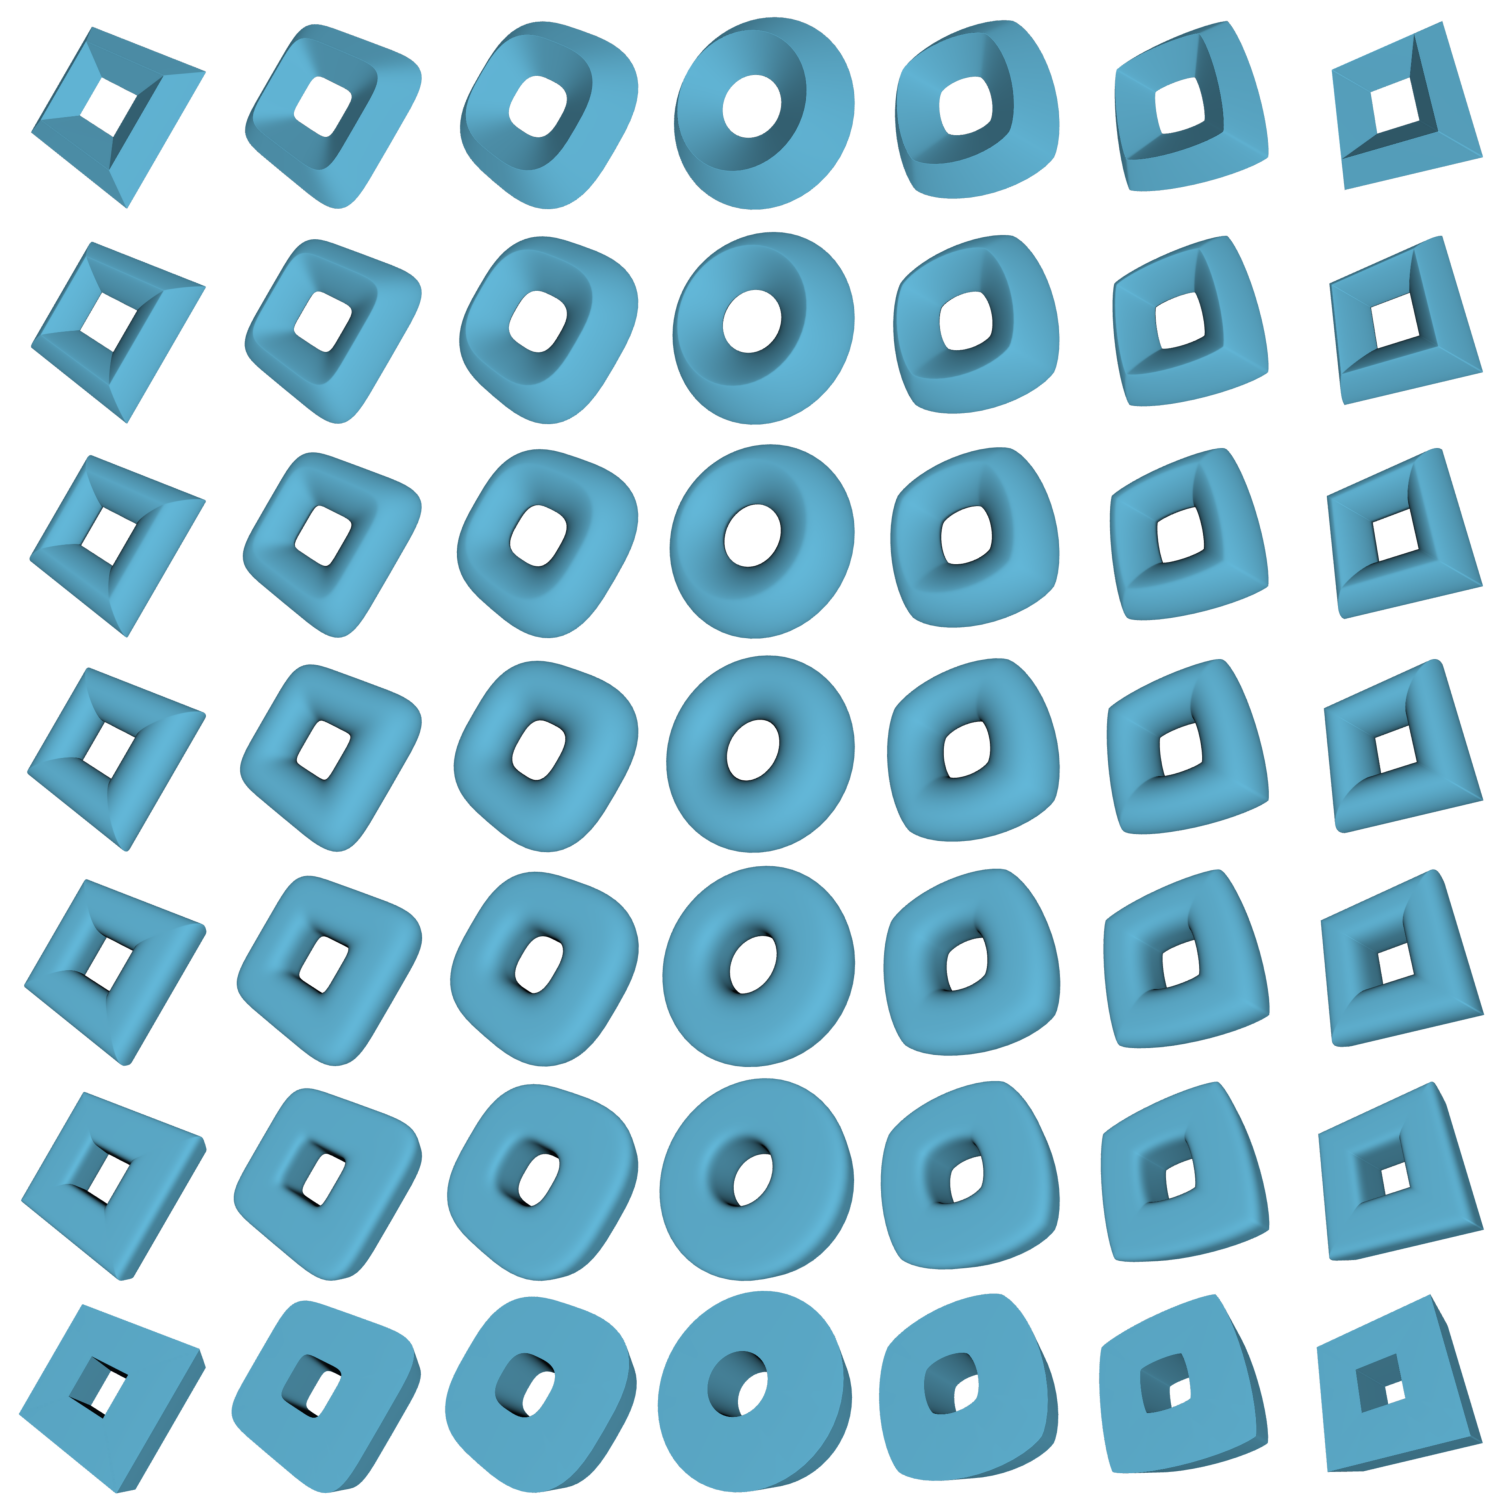
\includegraphics[width=\linewidth]{figs/topogen/toroids_overview.png}
  \caption{Different supertoroids obtained for fixed values of $a_i, i \in \{1, 2, 3\}$ and increasing values of $\epsilon_1$ (left to right) and $\epsilon_2$ (bottom to top). As mentioned in TO ADD, using these shapes for $k$-tori ($k \geq 2$) is challenging because they may not preserve the genus, for instance if some parts are too thin or sharp.}
  \label{fig:toroids-overview}
\end{figure}

\begin{figure}[t]
  \centering
  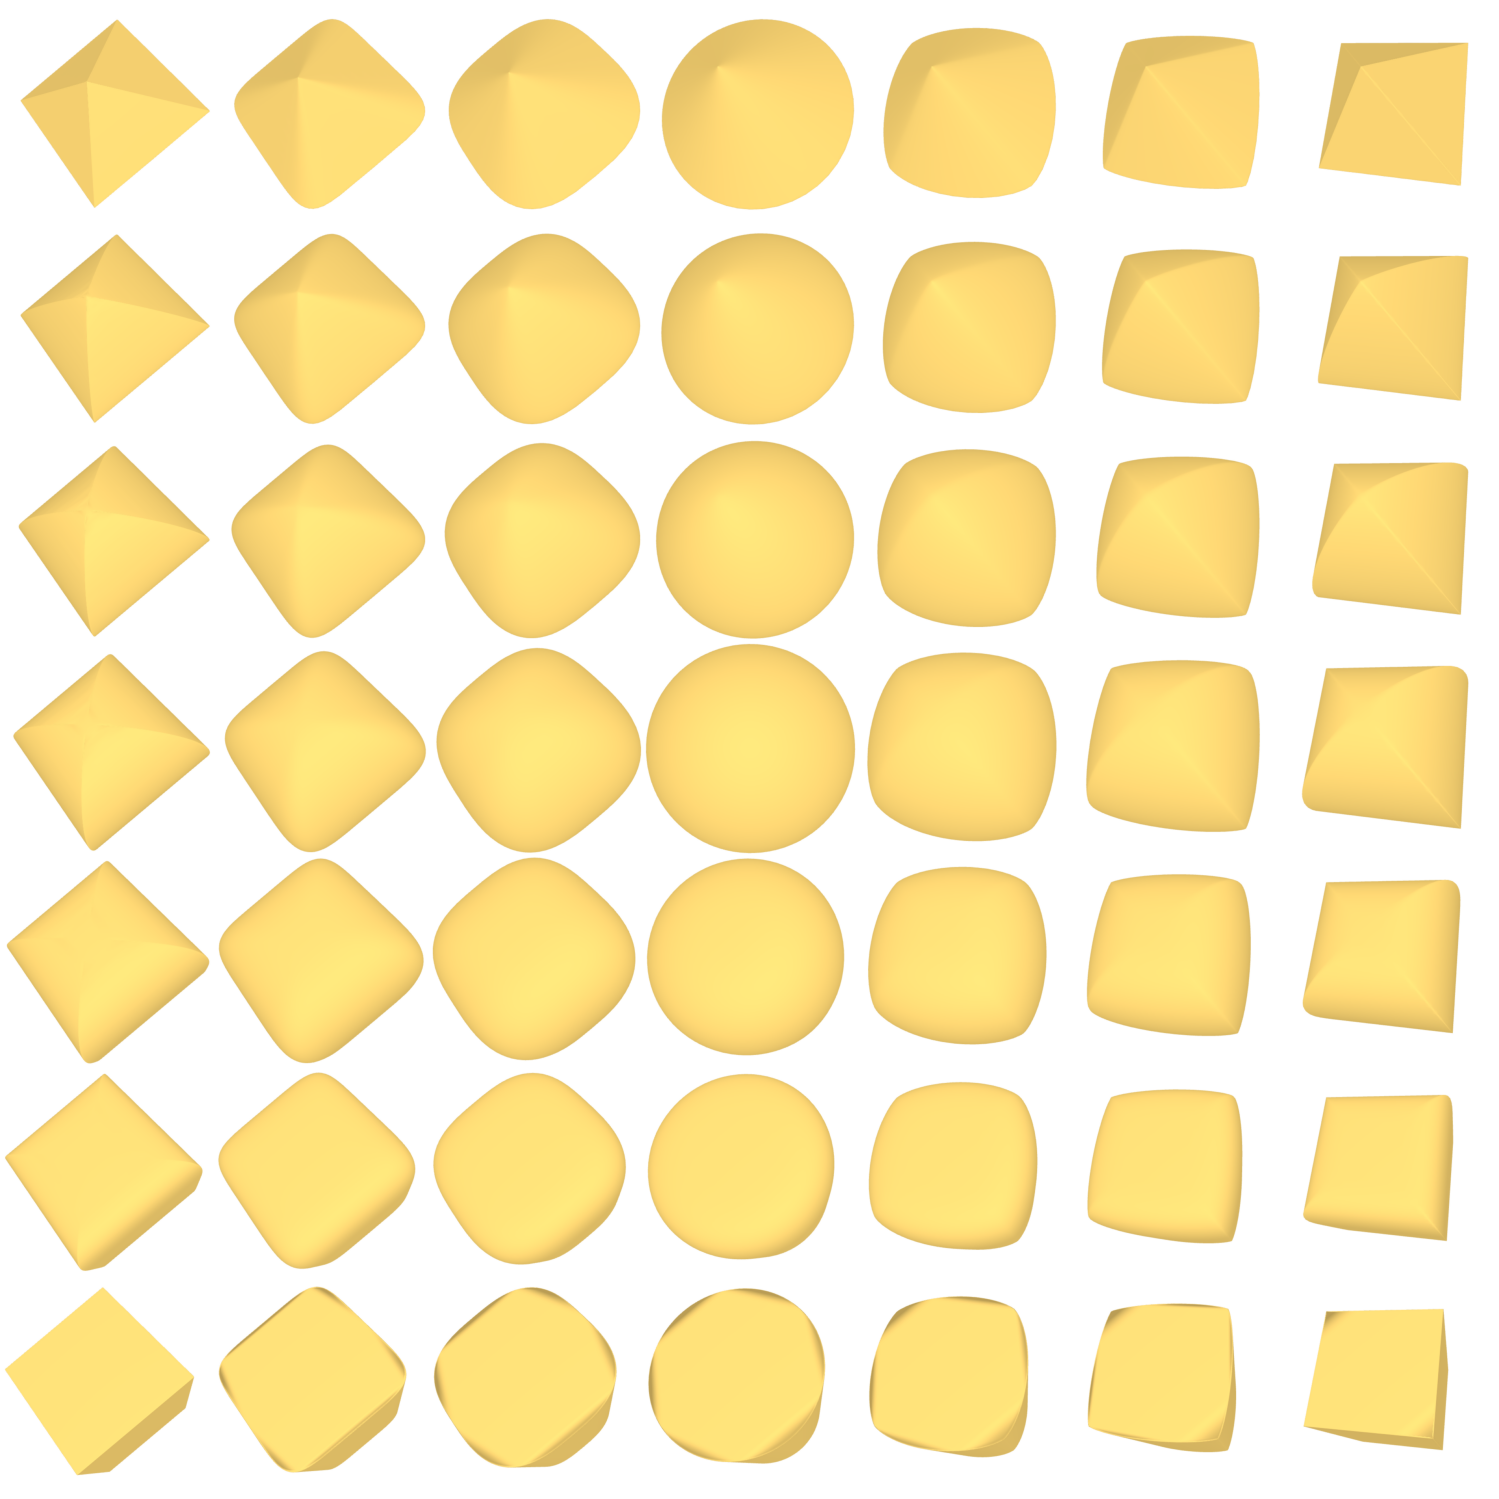
\includegraphics[width=\linewidth]{figs/topogen/ellipsoids_overview.png}
   \caption{Different superellipsoids obtained for fixed values of $a_i, i \in \{1, 2, 3\}$ and increasing values of $\epsilon_1$ (left to right) and $\epsilon_2$ (bottom to top).}
   \label{fig:ellipsoids-overview}
\end{figure}

\textbf{$K$-tori.} In the case of higher-genus meshes, there are no closed-form parametric equations. Instead, we leverage the implicit formulation of tori. A $k$-torus is generated by (1) evenly distributing tori on a circle, (2) blending their signed distance functions (SDF) through a smooth union operator, and finally (3) extracting the mesh via marching cubes with a grid-size. However, this process is more computationally intensive as it requires applying marching cubes the discretized SDF, whose complexity scales in $O(N^3)$ where $N$ is the grid size. And since we seek to have high quality meshes to preserve fine-grained details (here holes), we use a higher grid resolution.

To smoothly blend the SDF of each torus generated independently, we use the \textit{smooth minimum} operator:

\begin{equation}
\operatorname{softmin}_k(s_1, s_2, \dots, s_n) 
= -\frac{1}{k} \log \left( \sum_{i=1}^n e^{-k s_i} \right)
\end{equation}

Where $(s_1, s_2, \dots, s_n) \in \mathbb{R}^{(N^3)}$ are the SDF of individual tori and $k$ is a hyperparameter controlling the smoothness of the blending. This operator is applied voxel wise. In other words, each voxel of the blended SDF is assigned with the smooth minimum value of the individual SDF.

\begin{figure}[t]
  \centering
  \includegraphics[width=\linewidth]{figs/topogen/ktori_overview.png}
   \caption{\textbf{Degrees of freedom allowed on k-tori.}}
   \label{fig:ktori-overview}
\end{figure}


% All text must be in a two-column format.
% The total allowable size of the text area is $6\frac78$ inches (17.46 cm) wide by $8\frac78$ inches (22.54 cm) high.
% Columns are to be $3\frac14$ inches (8.25 cm) wide, with a $\frac{5}{16}$ inch (0.8 cm) space between them.
% The main title (on the first page) should begin 1 inch (2.54 cm) from the top edge of the page.
% The second and following pages should begin 1 inch (2.54 cm) from the top edge.
% On all pages, the bottom margin should be $1\frac{1}{8}$ inches (2.86 cm) from the bottom edge of the page for $8.5 \times 11$-inch paper;
% for A4 paper, approximately $1\frac{5}{8}$ inches (4.13 cm) from the bottom edge of the
% page.

% %-------------------------------------------------------------------------
% \subsection{Margins and page numbering}

% All printed material, including text, illustrations, and charts, must be kept
% within a print area $6\frac{7}{8}$ inches (17.46 cm) wide by $8\frac{7}{8}$ inches (22.54 cm)
% high.
% %
% Page numbers should be in the footer, centered and $\frac{3}{4}$ inches from the bottom of the page.
% The review version should have page numbers, yet the final version submitted as camera ready should not show any page numbers.
% The \LaTeX\ template takes care of this when used properly.



% %-------------------------------------------------------------------------
% \subsection{Type style and fonts}

% Wherever Times is specified, Times Roman may also be used.
% If neither is available on your word processor, please use the font closest in
% appearance to Times to which you have access.

% MAIN TITLE.
% Center the title $1\frac{3}{8}$ inches (3.49 cm) from the top edge of the first page.
% The title should be in Times 14-point, boldface type.
% Capitalize the first letter of nouns, pronouns, verbs, adjectives, and adverbs;
% do not capitalize articles, coordinate conjunctions, or prepositions (unless the title begins with such a word).
% Leave two blank lines after the title.

% AUTHOR NAME(s) and AFFILIATION(s) are to be centered beneath the title
% and printed in Times 12-point, non-boldface type.
% This information is to be followed by two blank lines.

% The ABSTRACT and MAIN TEXT are to be in a two-column format.

% MAIN TEXT.
% Type main text in 10-point Times, single-spaced.
% Do NOT use double-spacing.
% All paragraphs should be indented 1 pica (approx.~$\frac{1}{6}$ inch or 0.422 cm).
% Make sure your text is fully justified---that is, flush left and flush right.
% Please do not place any additional blank lines between paragraphs.

% Figure and table captions should be 9-point Roman type as in \cref{fig:onecol,fig:short}.
% Short captions should be centred.

% \noindent Callouts should be 9-point Helvetica, non-boldface type.
% Initially capitalize only the first word of section titles and first-, second-, and third-order headings.

% FIRST-ORDER HEADINGS.
% (For example, {\large \bf 1. Introduction}) should be Times 12-point boldface, initially capitalized, flush left, with one blank line before, and one blank line after.

% SECOND-ORDER HEADINGS.
% (For example, { \bf 1.1. Database elements}) should be Times 11-point boldface, initially capitalized, flush left, with one blank line before, and one after.
% If you require a third-order heading (we discourage it), use 10-point Times, boldface, initially capitalized, flush left, preceded by one blank line, followed by a period and your text on the same line.

% %-------------------------------------------------------------------------
% \subsection{Footnotes}

% Please use footnotes\footnote{This is what a footnote looks like.
% It often distracts the reader from the main flow of the argument.} sparingly.
% Indeed, try to avoid footnotes altogether and include necessary peripheral observations in the text (within parentheses, if you prefer, as in this sentence).
% If you wish to use a footnote, place it at the bottom of the column on the page on which it is referenced.
% Use Times 8-point type, single-spaced.


% %-------------------------------------------------------------------------
% \subsection{Cross-references}

% For the benefit of author(s) and readers, please use the
% {\small\begin{verbatim}
%   \cref{...}
% \end{verbatim}}  command for cross-referencing to figures, tables, equations, or sections.
% This will automatically insert the appropriate label alongside the cross-reference as in this example:
% \begin{quotation}
%   To see how our method outperforms previous work, please see \cref{fig:onecol} and \cref{tab:example}.
%   It is also possible to refer to multiple targets as once, \eg~to \cref{fig:onecol,fig:short-a}.
%   You may also return to \cref{sec:formatting} or look at \cref{eq:also-important}.
% \end{quotation}
% If you do not wish to abbreviate the label, for example at the beginning of the sentence, you can use the
% {\small\begin{verbatim}
%   \Cref{...}
% \end{verbatim}}
% command. Here is an example:
% \begin{quotation}
%   \Cref{fig:onecol} is also quite important.
% \end{quotation}

% %-------------------------------------------------------------------------
% \subsection{References}

% List and number all bibliographical references in 9-point Times, single-spaced, at the end of your paper.
% When referenced in the text, enclose the citation number in square brackets, for
% example~\cite{Authors14}.
% Where appropriate, include page numbers and the name(s) of editors of referenced books.
% When you cite multiple papers at once, please make sure that you cite them in numerical order like this \cite{Alpher02,Alpher03,Alpher05,Authors14b,Authors14}.
% If you use the template as advised, this will be taken care of automatically.

% \begin{table}
%   \centering
%   \begin{tabular}{@{}lc@{}}
%     \toprule
%     Method & Frobnability \\
%     \midrule
%     Theirs & Frumpy \\
%     Yours & Frobbly \\
%     Ours & Makes one's heart Frob\\
%     \bottomrule
%   \end{tabular}
%   \caption{Results.   Ours is better.}
%   \label{tab:example}
% \end{table}

% %-------------------------------------------------------------------------
% \subsection{Illustrations, graphs, and photographs}

% All graphics should be centered.
% In \LaTeX, avoid using the \texttt{center} environment for this purpose, as this adds potentially unwanted whitespace.
% Instead use
% {\small\begin{verbatim}
%   \centering
% \end{verbatim}}
% at the beginning of your figure.
% Please ensure that any point you wish to make is resolvable in a printed copy of the paper.
% Resize fonts in figures to match the font in the body text, and choose line widths that render effectively in print.
% Readers (and reviewers), even of an electronic copy, may choose to print your paper in order to read it.
% You cannot insist that they do otherwise, and therefore must not assume that they can zoom in to see tiny details on a graphic.

% When placing figures in \LaTeX, it's almost always best to use \verb+\includegraphics+, and to specify the figure width as a multiple of the line width as in the example below
% {\small\begin{verbatim}
%    \usepackage{graphicx} ...
%    \includegraphics[width=0.8\linewidth]
%                    {myfile.pdf}
% \end{verbatim}
% }


% %-------------------------------------------------------------------------
% \subsection{Color}

% Please refer to the author guidelines on the \confName\ \confYear\ web page for a discussion of the use of color in your document.

% If you use color in your plots, please keep in mind that a significant subset of reviewers and readers may have a color vision deficiency; red-green blindness is the most frequent kind.
% Hence avoid relying only on color as the discriminative feature in plots (such as red \vs green lines), but add a second discriminative feature to ease disambiguation.